%----------------------------------------------------------------------------
% solution_3_pulses.tex
% by Troy Hix, March 2005
%----------------------------------------------------------------------------
\begin{figure}
\centering
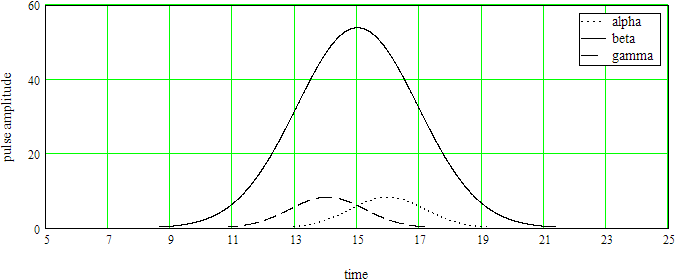
\includegraphics[width=5.00in]
{solution_3_pulses/solution_3_pulses.png}\\
\caption[Three color optimal pulse sequence]{Three color optimal pulse sequence. When $w=10^8$, the local optimum occurs when $\sigma_\alpha=\sigma_\gamma=2.84885872022$, $\sigma_\beta=4.59093152823$, $A=C=8.28793940926$ (5.093 times the area of the $\pi$--pulse), $B=53.8858080585$ (53.363 times the area of the $\pi$--pulse), and $\Delta_\alpha=\Delta_\gamma=-0.972655687674$.}
\label{solution three pulses}
\end{figure} 
%----------------------------------------------------------------------------

%----------------------------------------------------------------------------
%----------------------------------------------------------------------------
Suppose the solution, $\ket{\Psi}$, to (\ref{one dynamics}) is known at N+1 points from $t_0$ to $t_N$ where $t_i<t_j$ when $i<j$ $\forall$  $i,j \in \{0,1,\cdots,N\}$. Let $\ket{n}_i$ be the value of the nth component ($n \in \{ 0,1,2,3 \}$) of the solution, $\ket{\Psi}$, at time $t_i$. Consider the cost function
%----------------------------------------------------------------------------
%----------------------------------------------------------------------------
\begin{equation}
\Phi
=
w\Phi_{residue}
+
\Phi_{intermediate}
\label{three cost}
\end{equation}
%----------------------------------------------------------------------------
where
%----------------------------------------------------------------------------
\begin{equation}
\Phi_{residue}
=
P_0(t_N)
+
P_1(t_N)
+
P_2(t_N)
\label{three residue cost}
\end{equation}
%----------------------------------------------------------------------------
%----------------------------------------------------------------------------
% solution_3_energy_levels.tex
% by Troy Hix, April 2005
%----------------------------------------------------------------------------
\begin{figure}
\centering
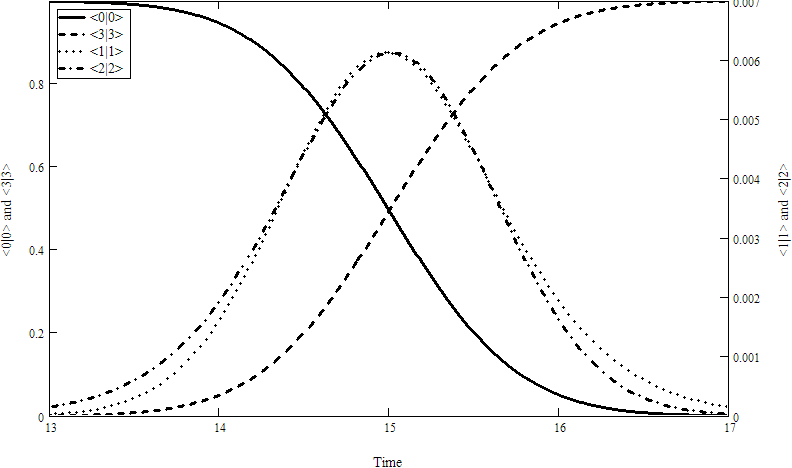
\includegraphics[width=5.00in]
{solution_3_energy_levels/solution_3_energy_levels.png}\\
\caption[Three color optimal solution]{Three color optimal solution. Occupation probability of the intermediate states $\ket{1}$ and $\ket{2}$ remain small while states $\ket{0}$ and $\ket{3}$ essentially exchange unity occupation probability in what looks like a single color $\pi$-pulse process (see figure \ref{solution one}).}
\label{solution three energy levels}
\end{figure} 
%----------------------------------------------------------------------------

%----------------------------------------------------------------------------
%----------------------------------------------------------------------------
\begin{equation}
\Phi_{intermediate}
=
\sum_i^N
P_1(t_i)
+
P_2(t_i)
\label{three int cost}
\end{equation}
%----------------------------------------------------------------------------
and $w$ is some weight factor.
%----------------------------------------------------------------------------
%----------------------------------------------------------------------------
A MathCAD program was written to minimize (\ref{three cost}) as a function of $\sigma_\alpha$, $\sigma_\beta$, $\sigma_\gamma$, $A$, $B$, $C$, $\Delta_\alpha$ and $\Delta_\gamma$. After some initial runs, some symmetries in the solutions prompted the following reduction of variables: $\sigma_\alpha=\sigma_\gamma$, $A=C$, $\Delta_\alpha=\Delta_\gamma$. Figure \ref{solution three pulses} shows the pulse sequence which minimized the cost function and figure \ref{solution three energy levels} shows the resulting motion in $\braket{\Psi}{\Psi}$.

In general, there are many local optima in the five dimensional solution space. It was found (with some exploring) that these optima generally improve with increasing amplitudes $A$, $B$, and $C$. Figure \ref{big solution three energy levels} show an example of one such solution. Note again the ``counter--intuitive'' pulse order of the first and last pulse.
%----------------------------------------------------------------------------
%----------------------------------------------------------------------------
% big_solution_3_energy_levels.tex
% by Troy Hix, April 2005
%----------------------------------------------------------------------------
\begin{figure}
\centering
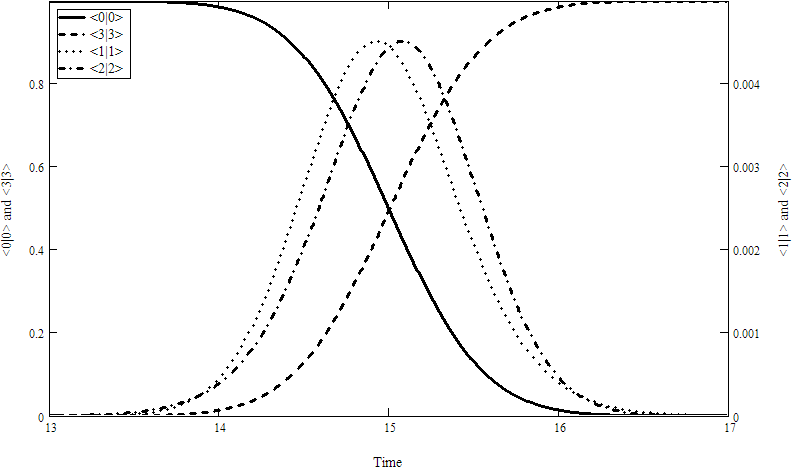
\includegraphics[width=5.00in]
{big_solution_3_energy_levels/big_solution_3_energy_levels.png}\\
\caption[Three color optimal solution - increased pulse amplitude]{Three color optimal solution - increased pulse amplitude. The local optimum ($w=10^8$) occurs when $\sigma_\alpha=\sigma_\gamma=2.19612383897$, $\sigma_\beta=4.57812933276$, $A=C=15.8819988348$ (7.524 times the area of the $\pi$--pulse), $B=101.198555496$ (99.937 times the area of the $\pi$--pulse), and $\Delta_\alpha=\Delta_\gamma=-0.93886228288$.}
\label{big solution three energy levels}
\end{figure} 
%----------------------------------------------------------------------------

%----------------------------------------------------------------------------
%----------------------------------------------------------------------------
%----------------------------------------------------------------------------
